\documentclass[border=14pt,tikz,dvipsnames]{standalone}

\usepackage{amsmath,amssymb} % for \text
\usepackage{physics} % for \abs
\usepackage{xspace} % for \xspace
\usepackage{bm} % for bold math \bm
\usepackage{setspace} \doublespacing

\usetikzlibrary{positioning} % for position relative to node
\usetikzlibrary{arrows.meta} % for arrow size
\usetikzlibrary{calc} % for computing coordinates
\tikzset{>=latex} % set default arrow head as latex

% TIKZ STUFF
\tikzstyle{mysmallarrow}=[-{Latex[length=6,width=6]},#1!80!black,thick,line width=1.6]
\def\connect[#1](#2)!#3!(#4){
  \draw[#1] (#2) |- ($(#2)!#3!(#4)$) node[pos=0.5] (#2-#4-1) {}
  -| (#4) node[pos=0.5] (#2-#4-2) {}
}
\colorlet{mywhite}{white!0!black}
\colorlet{myred}{red!80!black}
\colorlet{myblue}{blue!80!black}
\colorlet{mygreen}{green!50!black}
\colorlet{myorange}{orange!80!yellow!90!red!90!black}
\tikzstyle{mycomment}=[inner sep=1pt,scale=1,align=left]
\tikzstyle{mybox}=[draw,#1!80!black,fill=#1!95!black!20,inner sep=5pt,outer sep=3pt,
                   thick,rounded corners=3pt,align=center,font=\bfseries]
\tikzstyle{mysmallbox}=[mybox=#1,outer sep=1.5pt]
\tikzstyle{myarrow}=[-{Latex[length=8,width=8]},#1!80!black,thick,line cap=round,line width=2]

% Informal visualization of the divide-and-conquer tree
\begin{document}

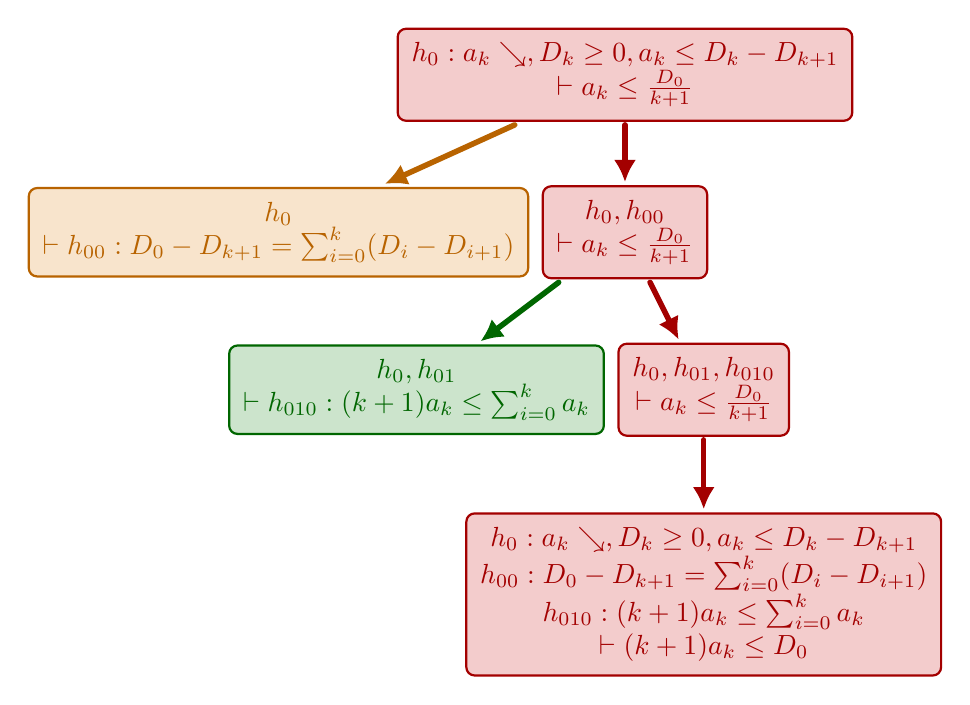
\begin{tikzpicture}[scale=1]
  \def\h{2} % vertical space between rows
  \def\w{2.3} % horizontal space between two main branches
  
  % 0
  \node[mysmallbox=myred] (0) at (0,0) {
  	$h_0: a_k \searrow , D_k \ge 0, a_k \le D_k - D_{k+1}$ \\
    $ \vdash a_k \le \frac{D_0}{k+1}$
   };
  
  % 01
  \path (0)++(0,-\h) node[mysmallbox=myred] (01) {
    $h_0, h_{00}$ \\
    $\vdash a_k \le \frac{D_0}{k+1} $
   };
  \draw[myarrow=myred] (0) -- (01);

  % 00
  \node[mysmallbox=myorange, left=\w pt of 01] (00) {
    $h_0$ \\
    $\vdash h_{00}: D_0 - D_{k+1} = \sum_{i=0}^k (D_i - D_{i+1}) $
   };
%  \node[mycomment, below=\w pt of 00] {
%    $h_0: D_0 - D_{k+1} = \sum_{i=0}^k (D_i - D_{i+1})$
%   };
  \draw[myarrow=myorange] (0) -- (00);
  
  % 011
  \path (01)++(1,-\h) node[mysmallbox=myred] (011) {
    $h_0, h_{01}, h_{010}$ \\
    $\vdash a_k \le \frac{D_0}{k+1} $
  };
  \draw[myarrow=myred] (01) -- (011);
  
  % 010
  \node[mysmallbox=mygreen, left=\w pt of 011] (010) {
    $h_0, h_{01}$ \\
    $\vdash h_{010}: (k+1) a_k \le \sum_{i=0}^k a_k $
  };  \draw[myarrow=mygreen] (01) -- (010);
  
  %\sum_{i=0}^k (D_i - D_{i+1}) \ge \sum_{i=0}^{k} a_i
  
  % 0110
  \path (011)++(0,-1.3*\h) node[mysmallbox=myred] (0110) {
    $h_0: a_k \searrow , D_k \ge 0, a_k \le D_k - D_{k+1}$ \\
    $h_{00}: D_0 - D_{k+1} = \sum_{i=0}^k (D_i - D_{i+1}) $ \\
    $h_{010}: (k+1) a_k \le \sum_{i=0}^k a_k$ \\
    $\vdash (k+1) a_k \le D_0 $
  };
  \draw[myarrow=myred] (011) -- (0110);
  
  % ARROWS
  %\connect[mysmallarrow=myorange](O.-95)!0.3!(0j);
  
  % LABELS
%  \node[mycomment,below=-1pt] at (O-0j-1.south) {%
%    jet $\pt>50\GeV$};
%  \node[mycomment,right=0pt of 1j] {%
%    $\mvis>100\GeV$};
  
\end{tikzpicture}

\end{document}